\section{Aspects organisationnels}
        \subsection{Niveau structurel}
        L'entreprise n'a pas besoin d'être restructurée au niveau des services. En effet, les services existants sont capables d'assurer le bon fonctionnement de GSTP. Un unique service a été créé, il s'agit de celui de location qui sera en charge de prendre en compte toutes les demandes de location des clients, puis de vérifier la disponibilité du matériel sur le délai de location demandé par un client. Ceci afin de vérifier si le matériel restera immobile durant cette période, sinon le service ne permettra pas la sortie de ce matériel. en effet le but premier reste de satisfaire les demandes de nos chantiers et non de louer un maximum de matériels.\\
        
         Cependant, nous avons décidé à des fins de réduction des coûts logistiques, de créer 4 sites secondaires en plus de celui du siège, chacun de ces sites comportera un dépôt de matériels (parc matériel), un magasin de pièces de rechange et un atelier de maintenance. Ce choix implique de remettre en cause l'organisation du personnel du département maintenance (service maintenance). En effet ce dernier disposait de 60 membres (dont 8 sur le siège) et le reste repartit sur les 40 chantiers. Mais le suivi était plus que critique, voir inexistant. Pour optimiser l'activité du département, nous avons décidé de revoir cette organisation. Ainsi les 8 personnes situés sur le siège pourront y rester. Parmi les autres, il faudra trouver des personnes ayant des compétences leur permettant de gérer le dépôt matériel ou le dépôt de pièces de rechange des 4 nouveaux sites. Ainsi parmi ces personnes, 8 personnes seront sélectionnés pour occuper ces postes ou la direction des ressources humaines devra effectuer un recrutement. Pour les autres salariés du département,
10 seront affectés par site secondaire à l'atelier de maintenance. Les employés n'ayant pas pu être réaffectés seront mis à la disposition des ressources humaines afin qu'ils puissent les affecter à d'autres services.\\

Une fois un chantier fini, le matériel sera transporté vers le nouveau chantier si aucune maintenance préventive n'est prévu sans repasser par le siège ou un site secondaire.

        \subsection{Niveau Processus}
        Après avoir défini l'ensemble de nos thèmes de progrès, il est apparu clairement un besoin de mettre à jour les modèles de processus existants. Nous avons mis à jour les principaux processus.\\

                \subsubsection{Processus Achat}
                    %Ci-dessous le modèle conceptuel de traitement (MCT). --> 
                    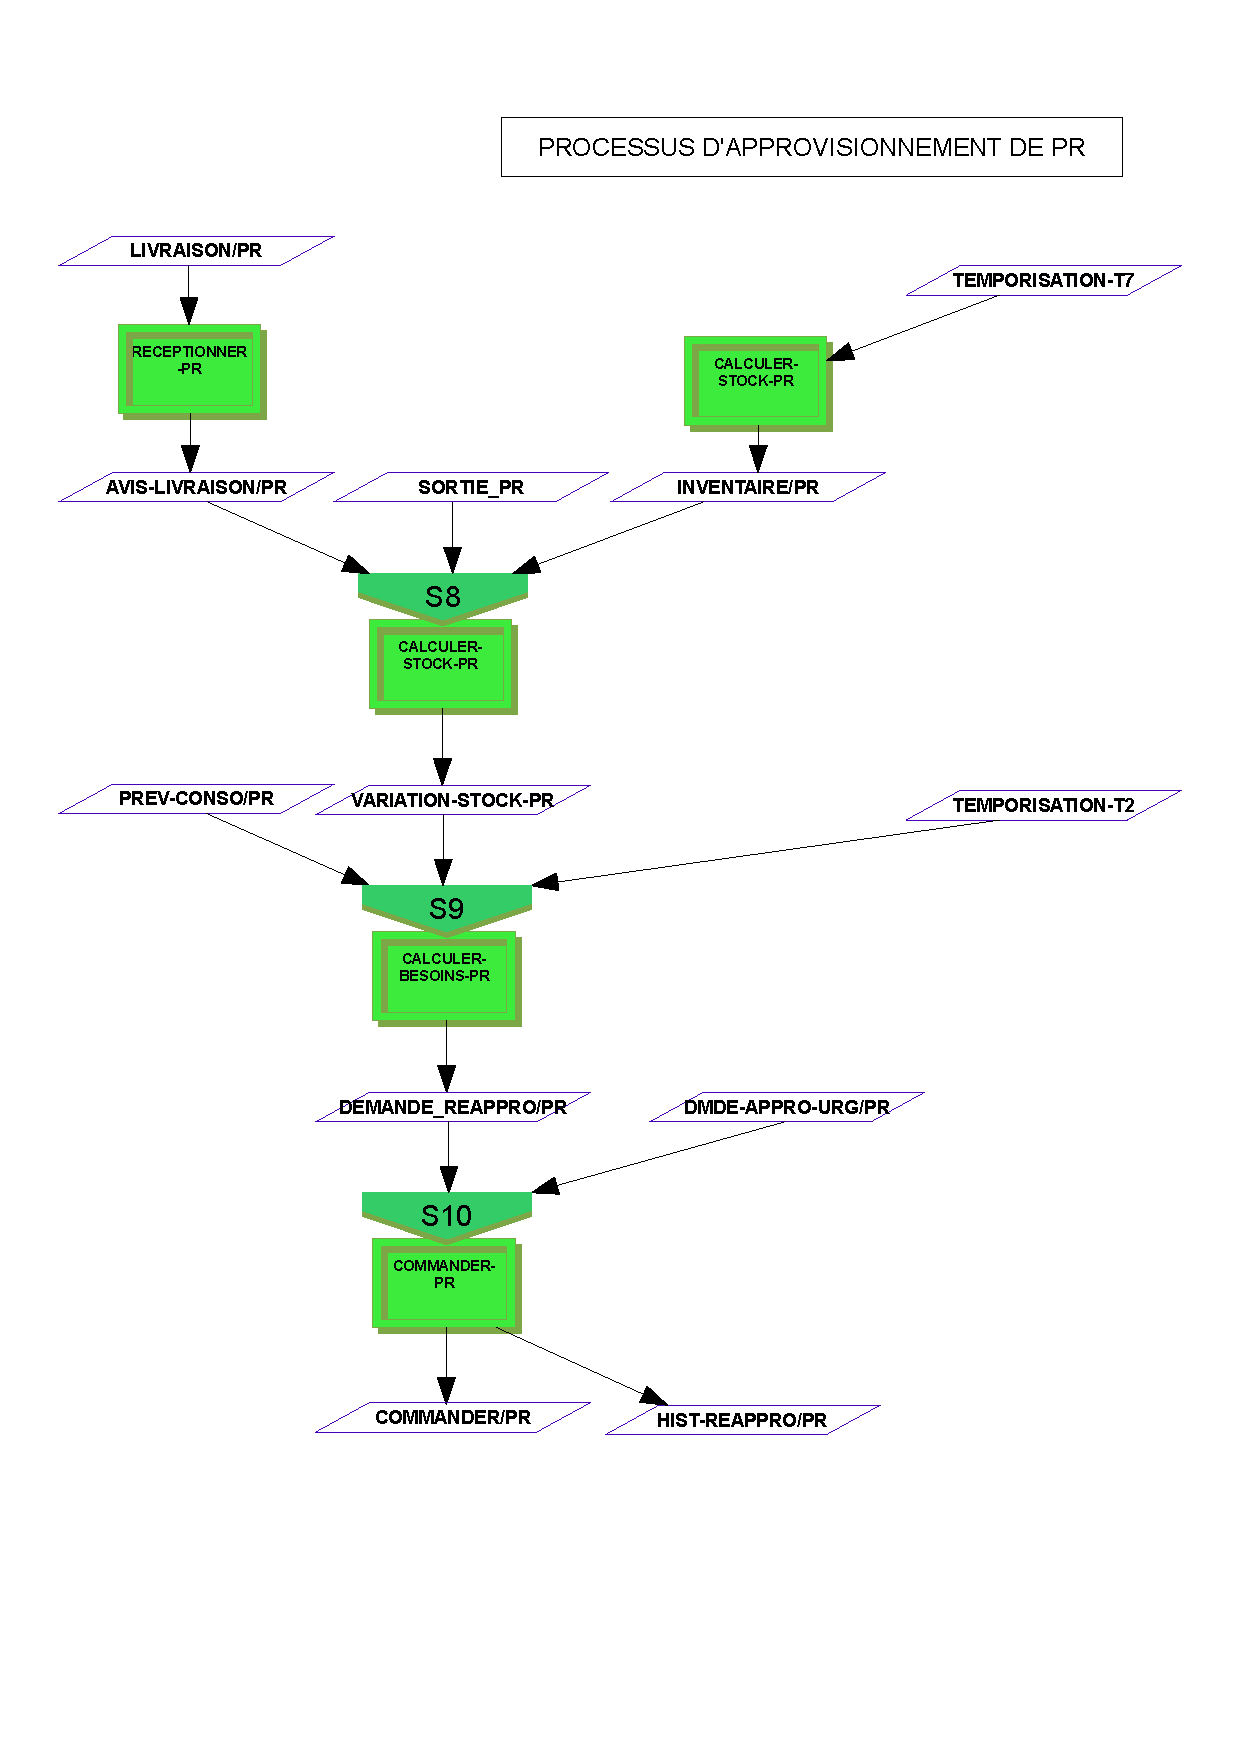
\includegraphics[width=0.9\textwidth]{approvisionnementdepr.pdf}

                    %Ci-dessous le modèle organisationnel de traitement (MOT). --> 
                    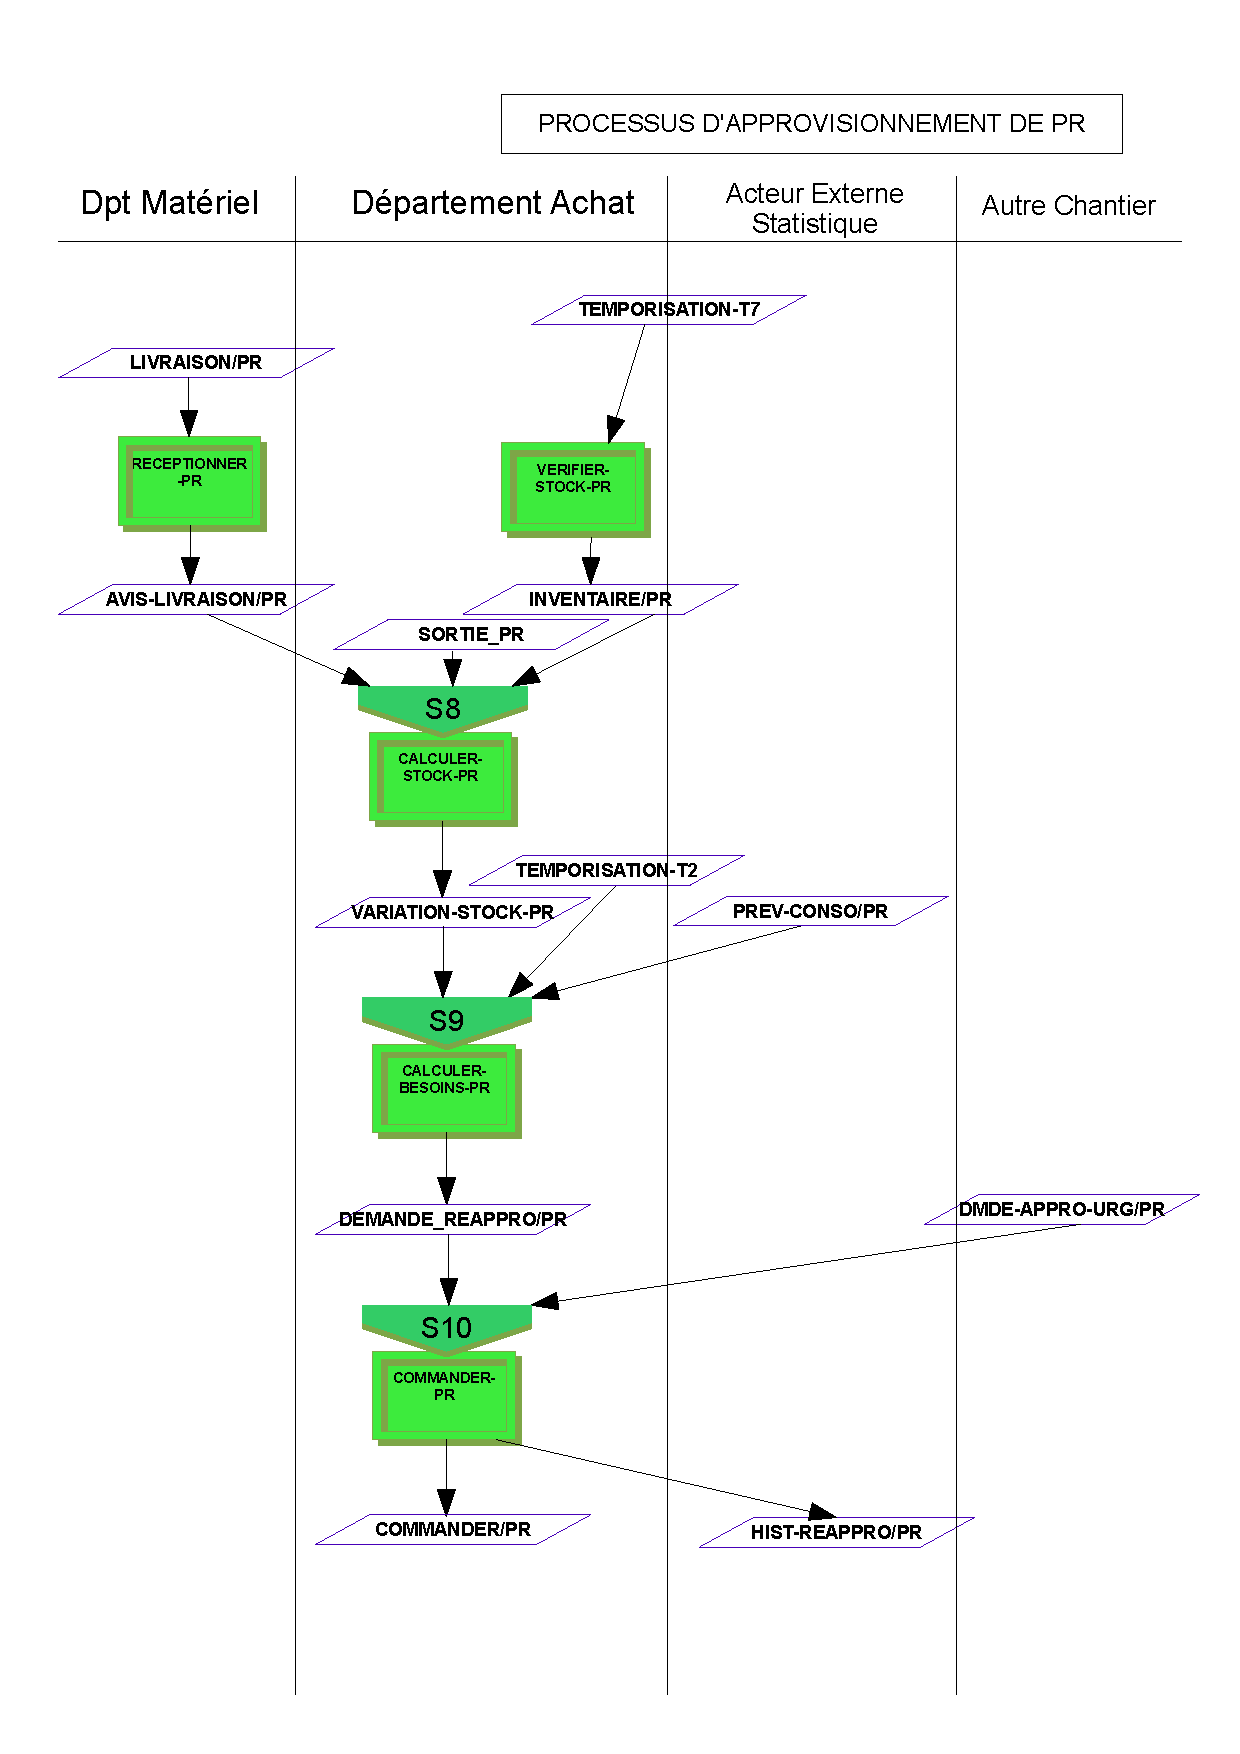
\includegraphics[width=0.9\textwidth]{MOTapprovisionnementdepr.pdf}

                \subsubsection{Processus Planification}
                    %Ci-dessous le modèle conceptuel de traitement (MCT). --> 
                    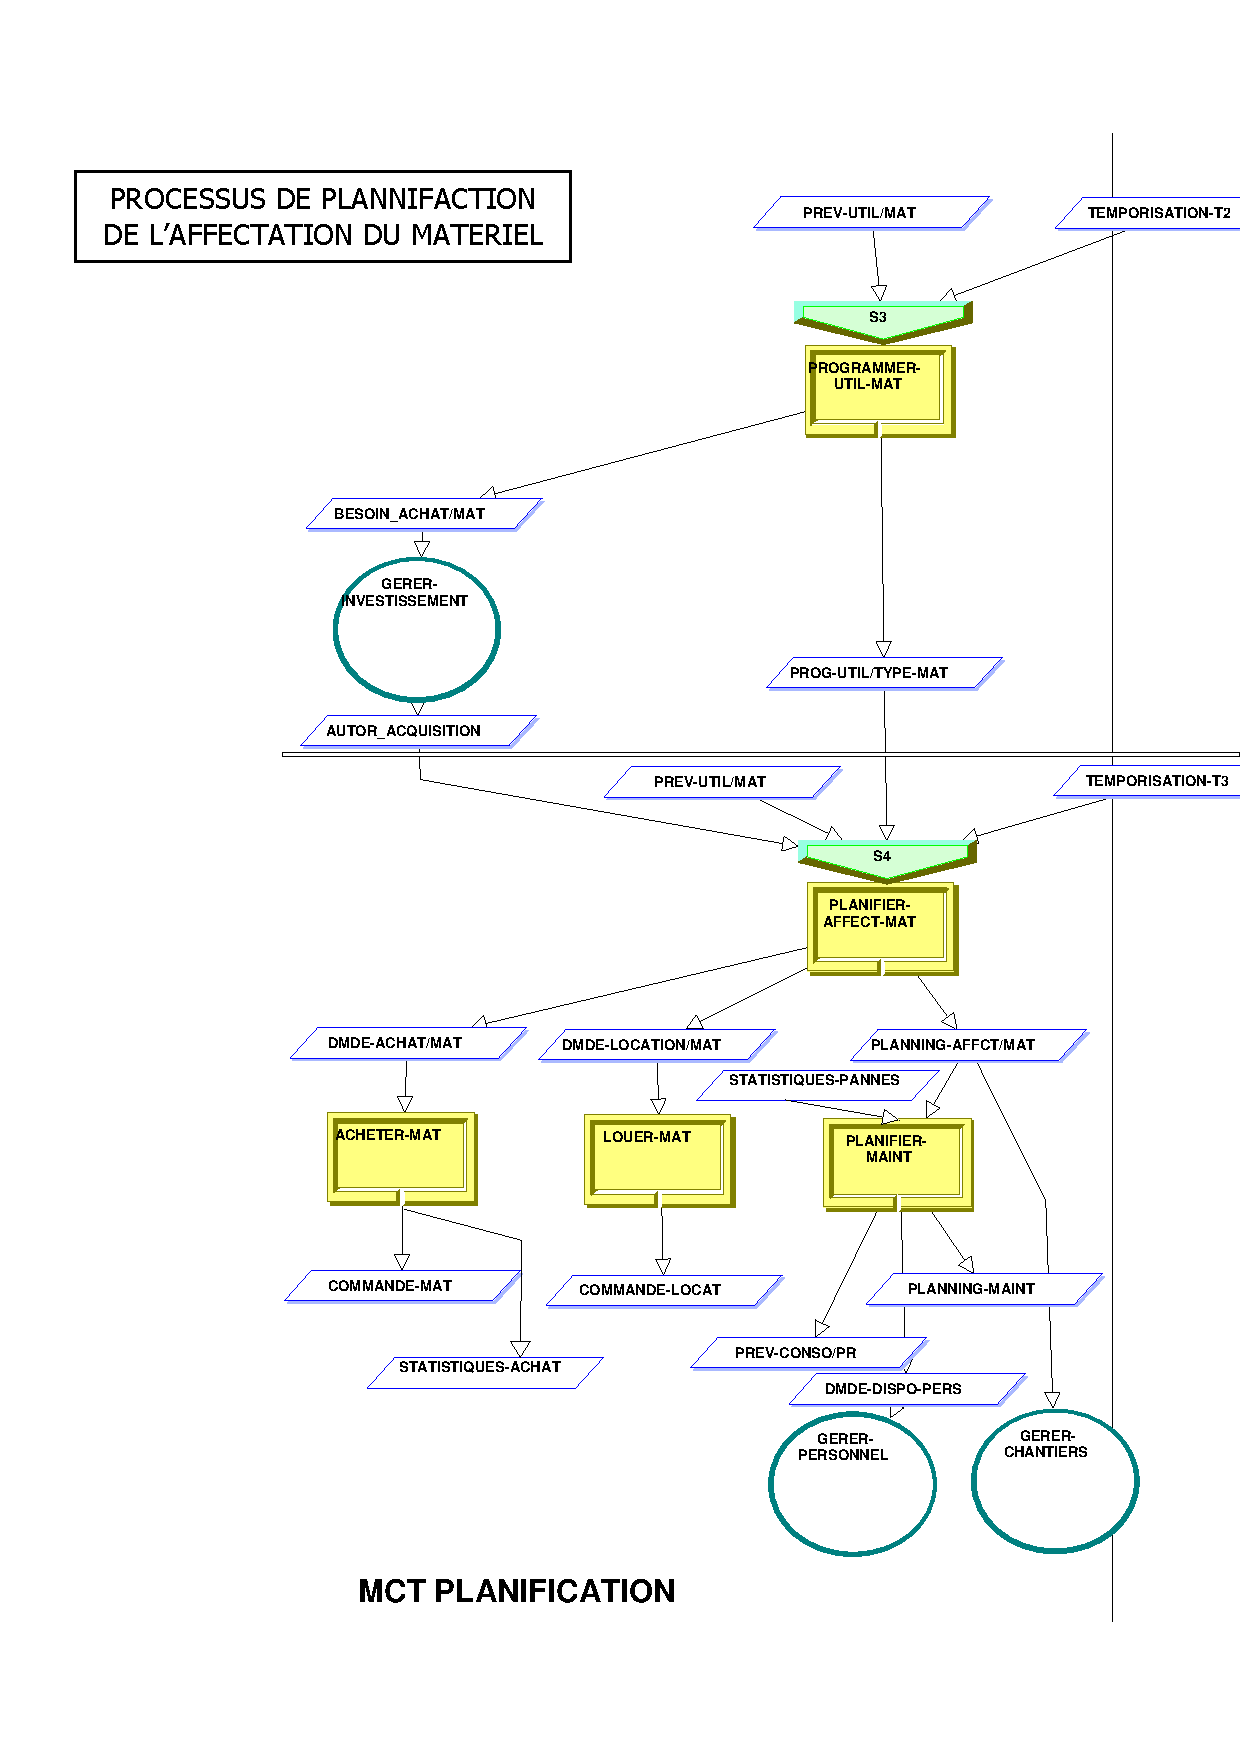
\includegraphics[width=0.9\textwidth]{planification.pdf}
                    
                    %Ci-dessous le modèle organisationnel de traitement (MOT). -->
                    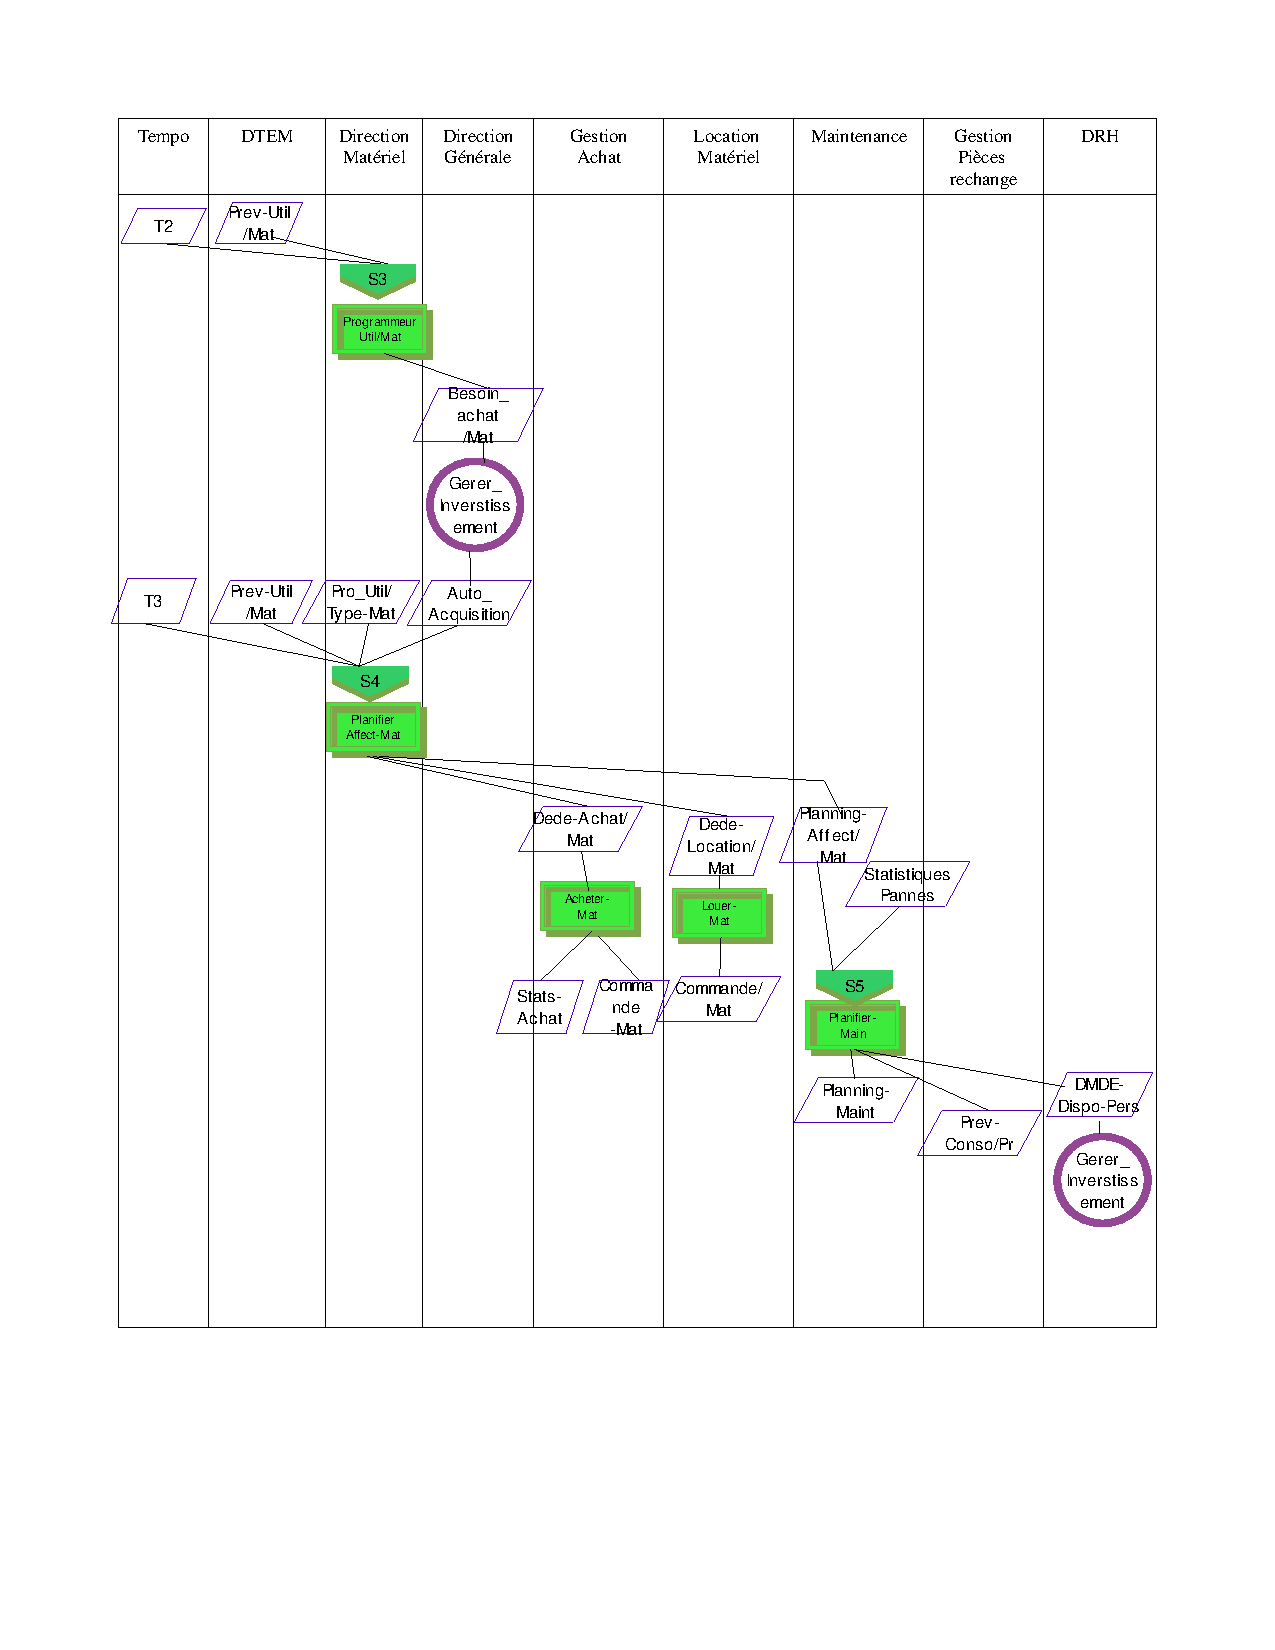
\includegraphics[width=0.9\textwidth]{MOTplanification.pdf}
                
                \subsubsection{Processus Affectation/Restitution de matériels}
                    %Ci-dessous le modèle conceptuel de traitement (MCT). --> 
                    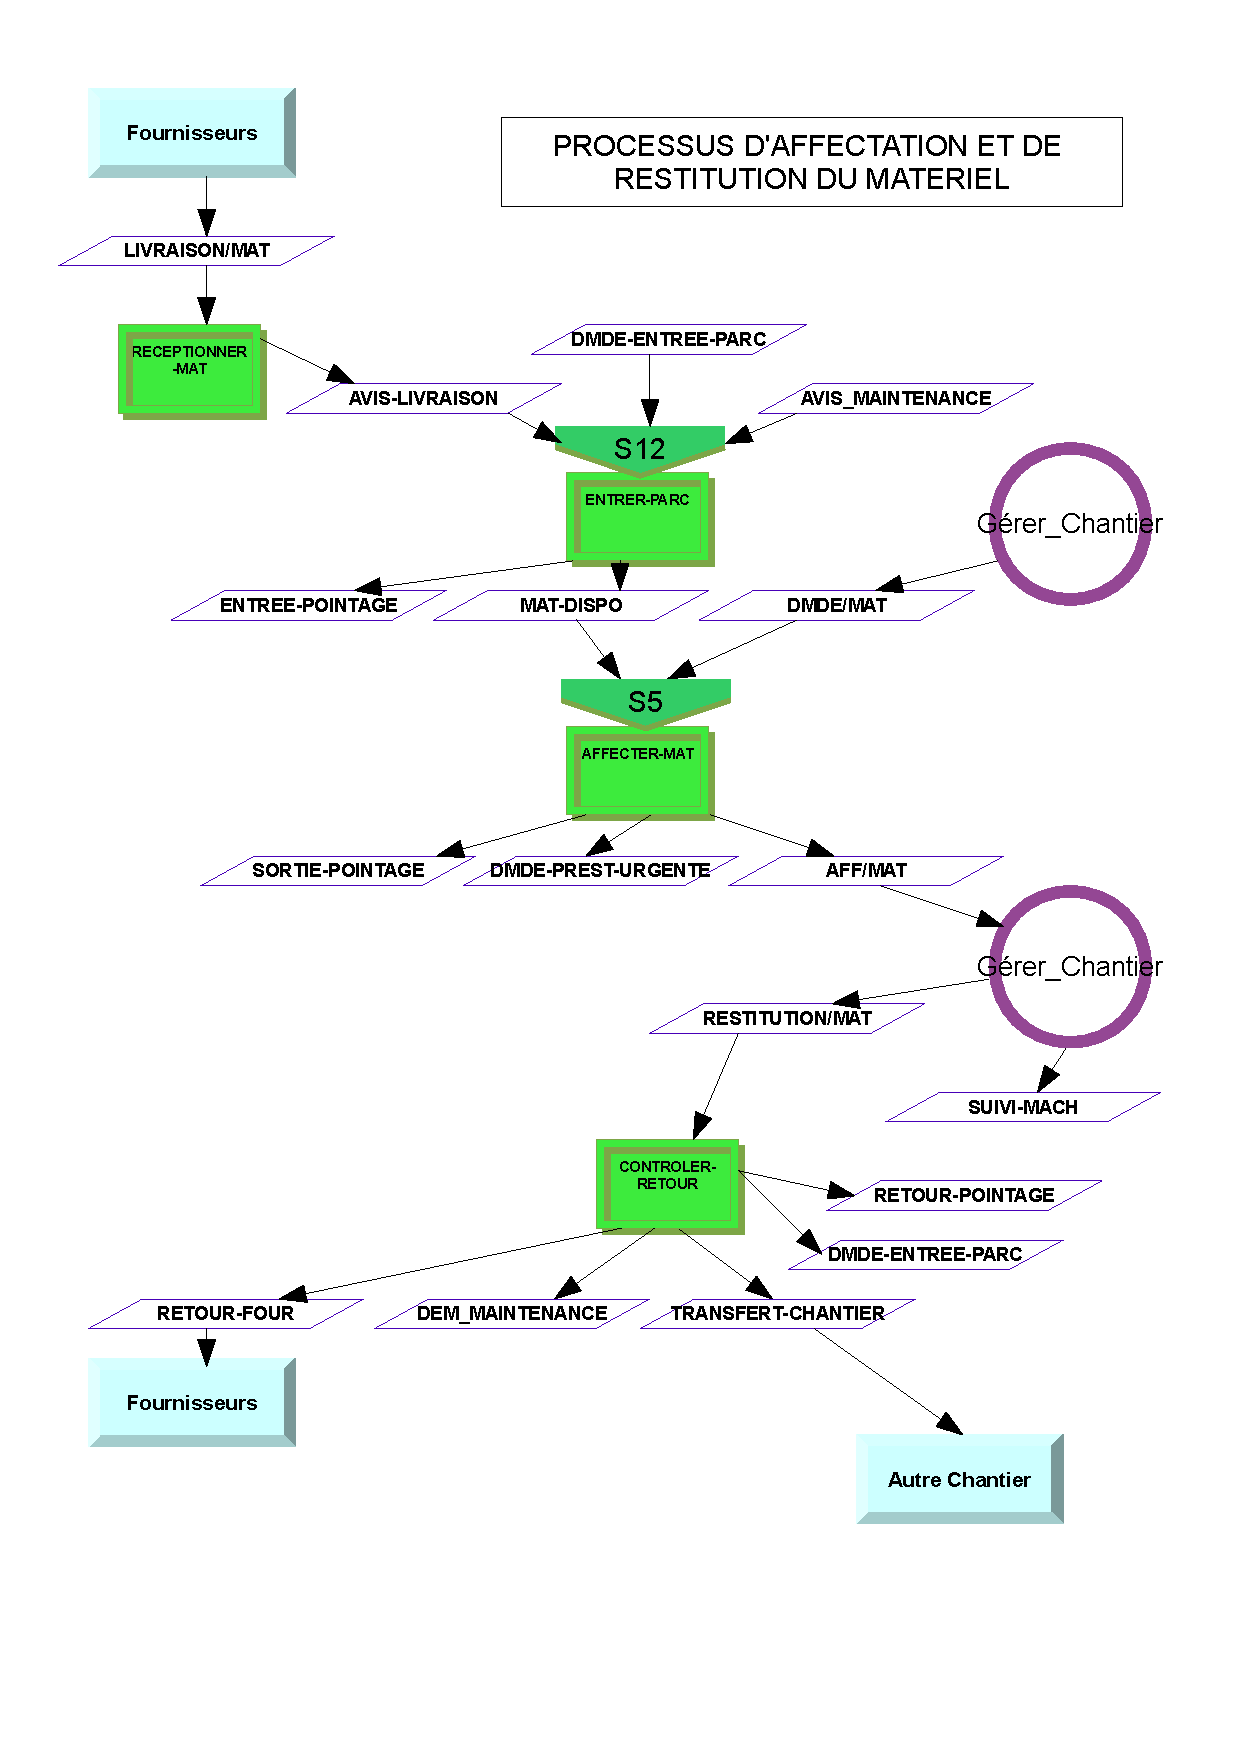
\includegraphics[width=0.9\textwidth]{affectationmateriel.pdf}

                    %Ci-dessous le modèle organisationnel de traitement (MOT). --> 
                    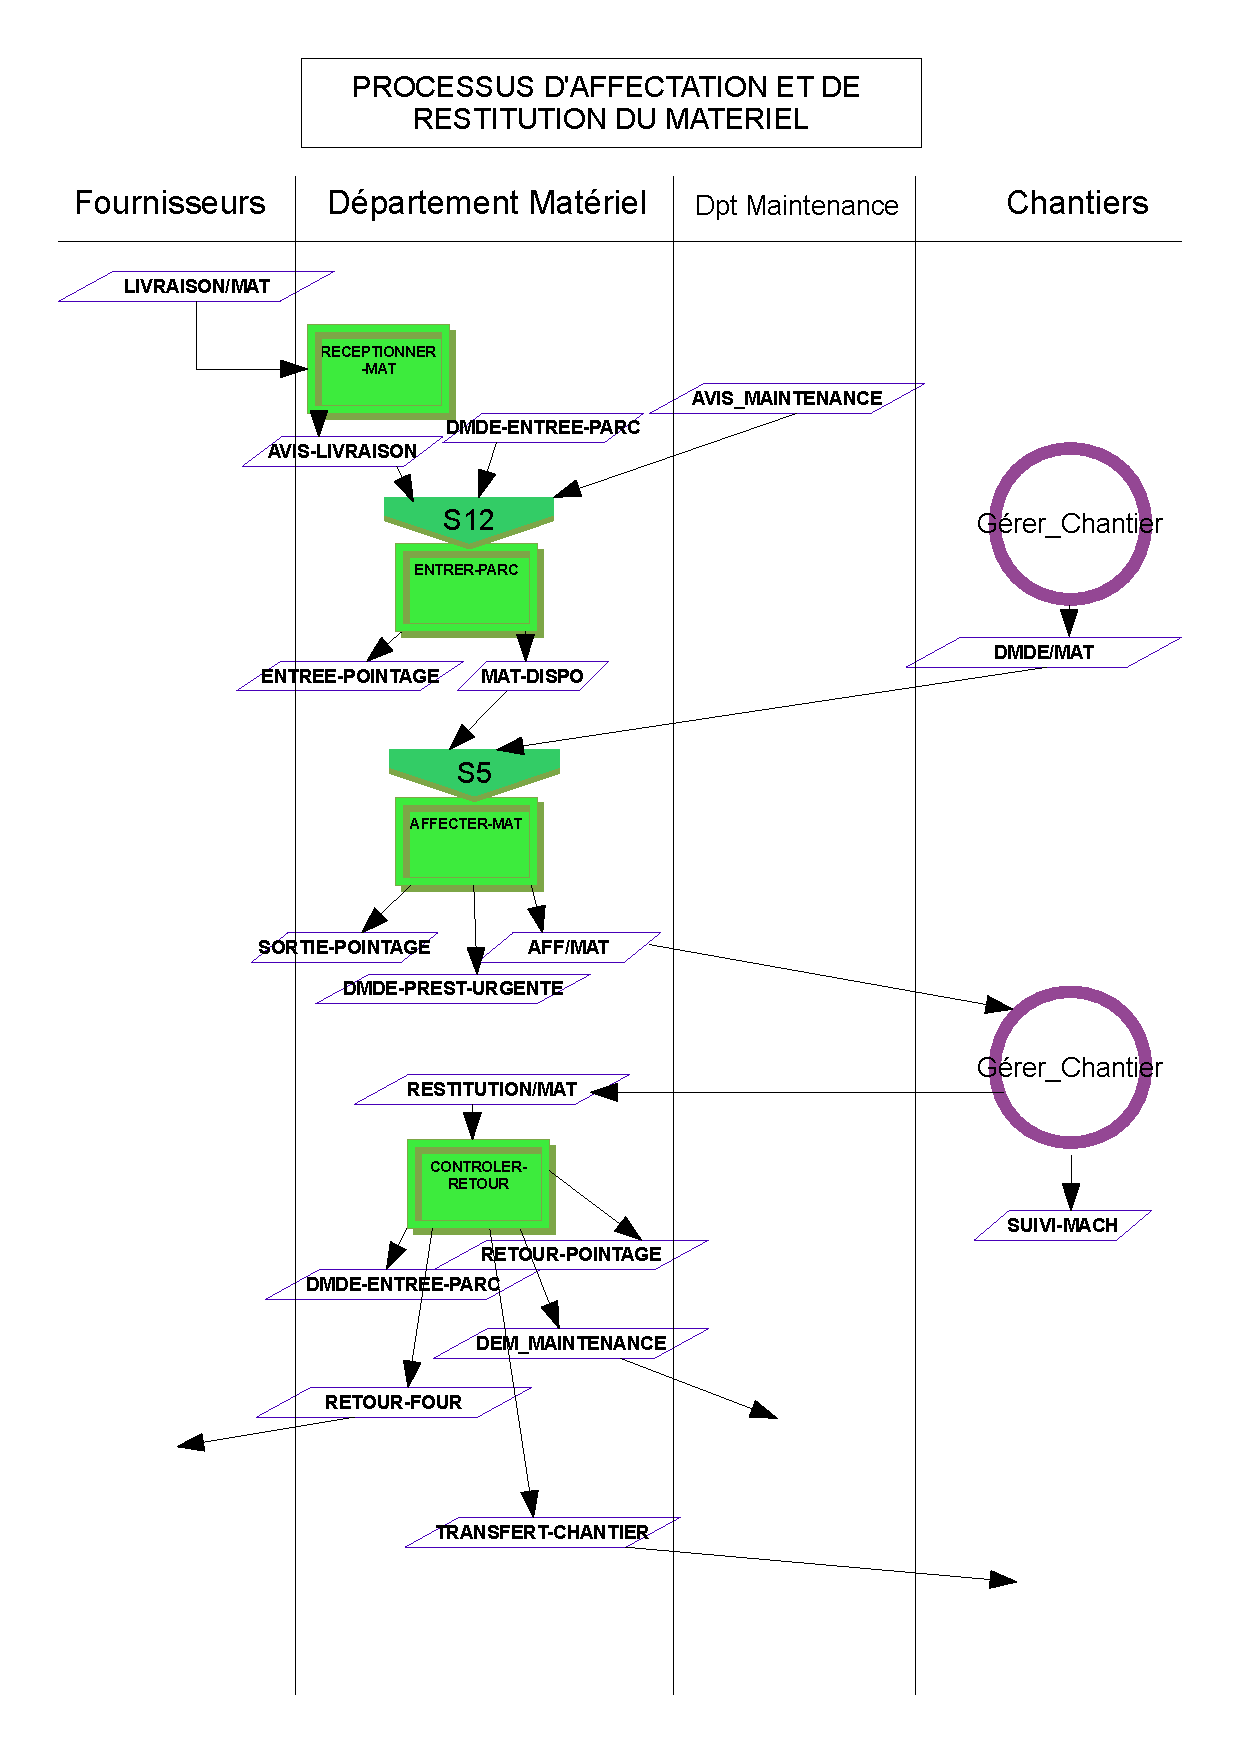
\includegraphics[width=0.9\textwidth]{MOTaffectationmateriel.pdf}

                \subsubsection{Processus Facturation}
                    %Ci-dessous le modèle conceptuel de traitement (MCT). --> 
                    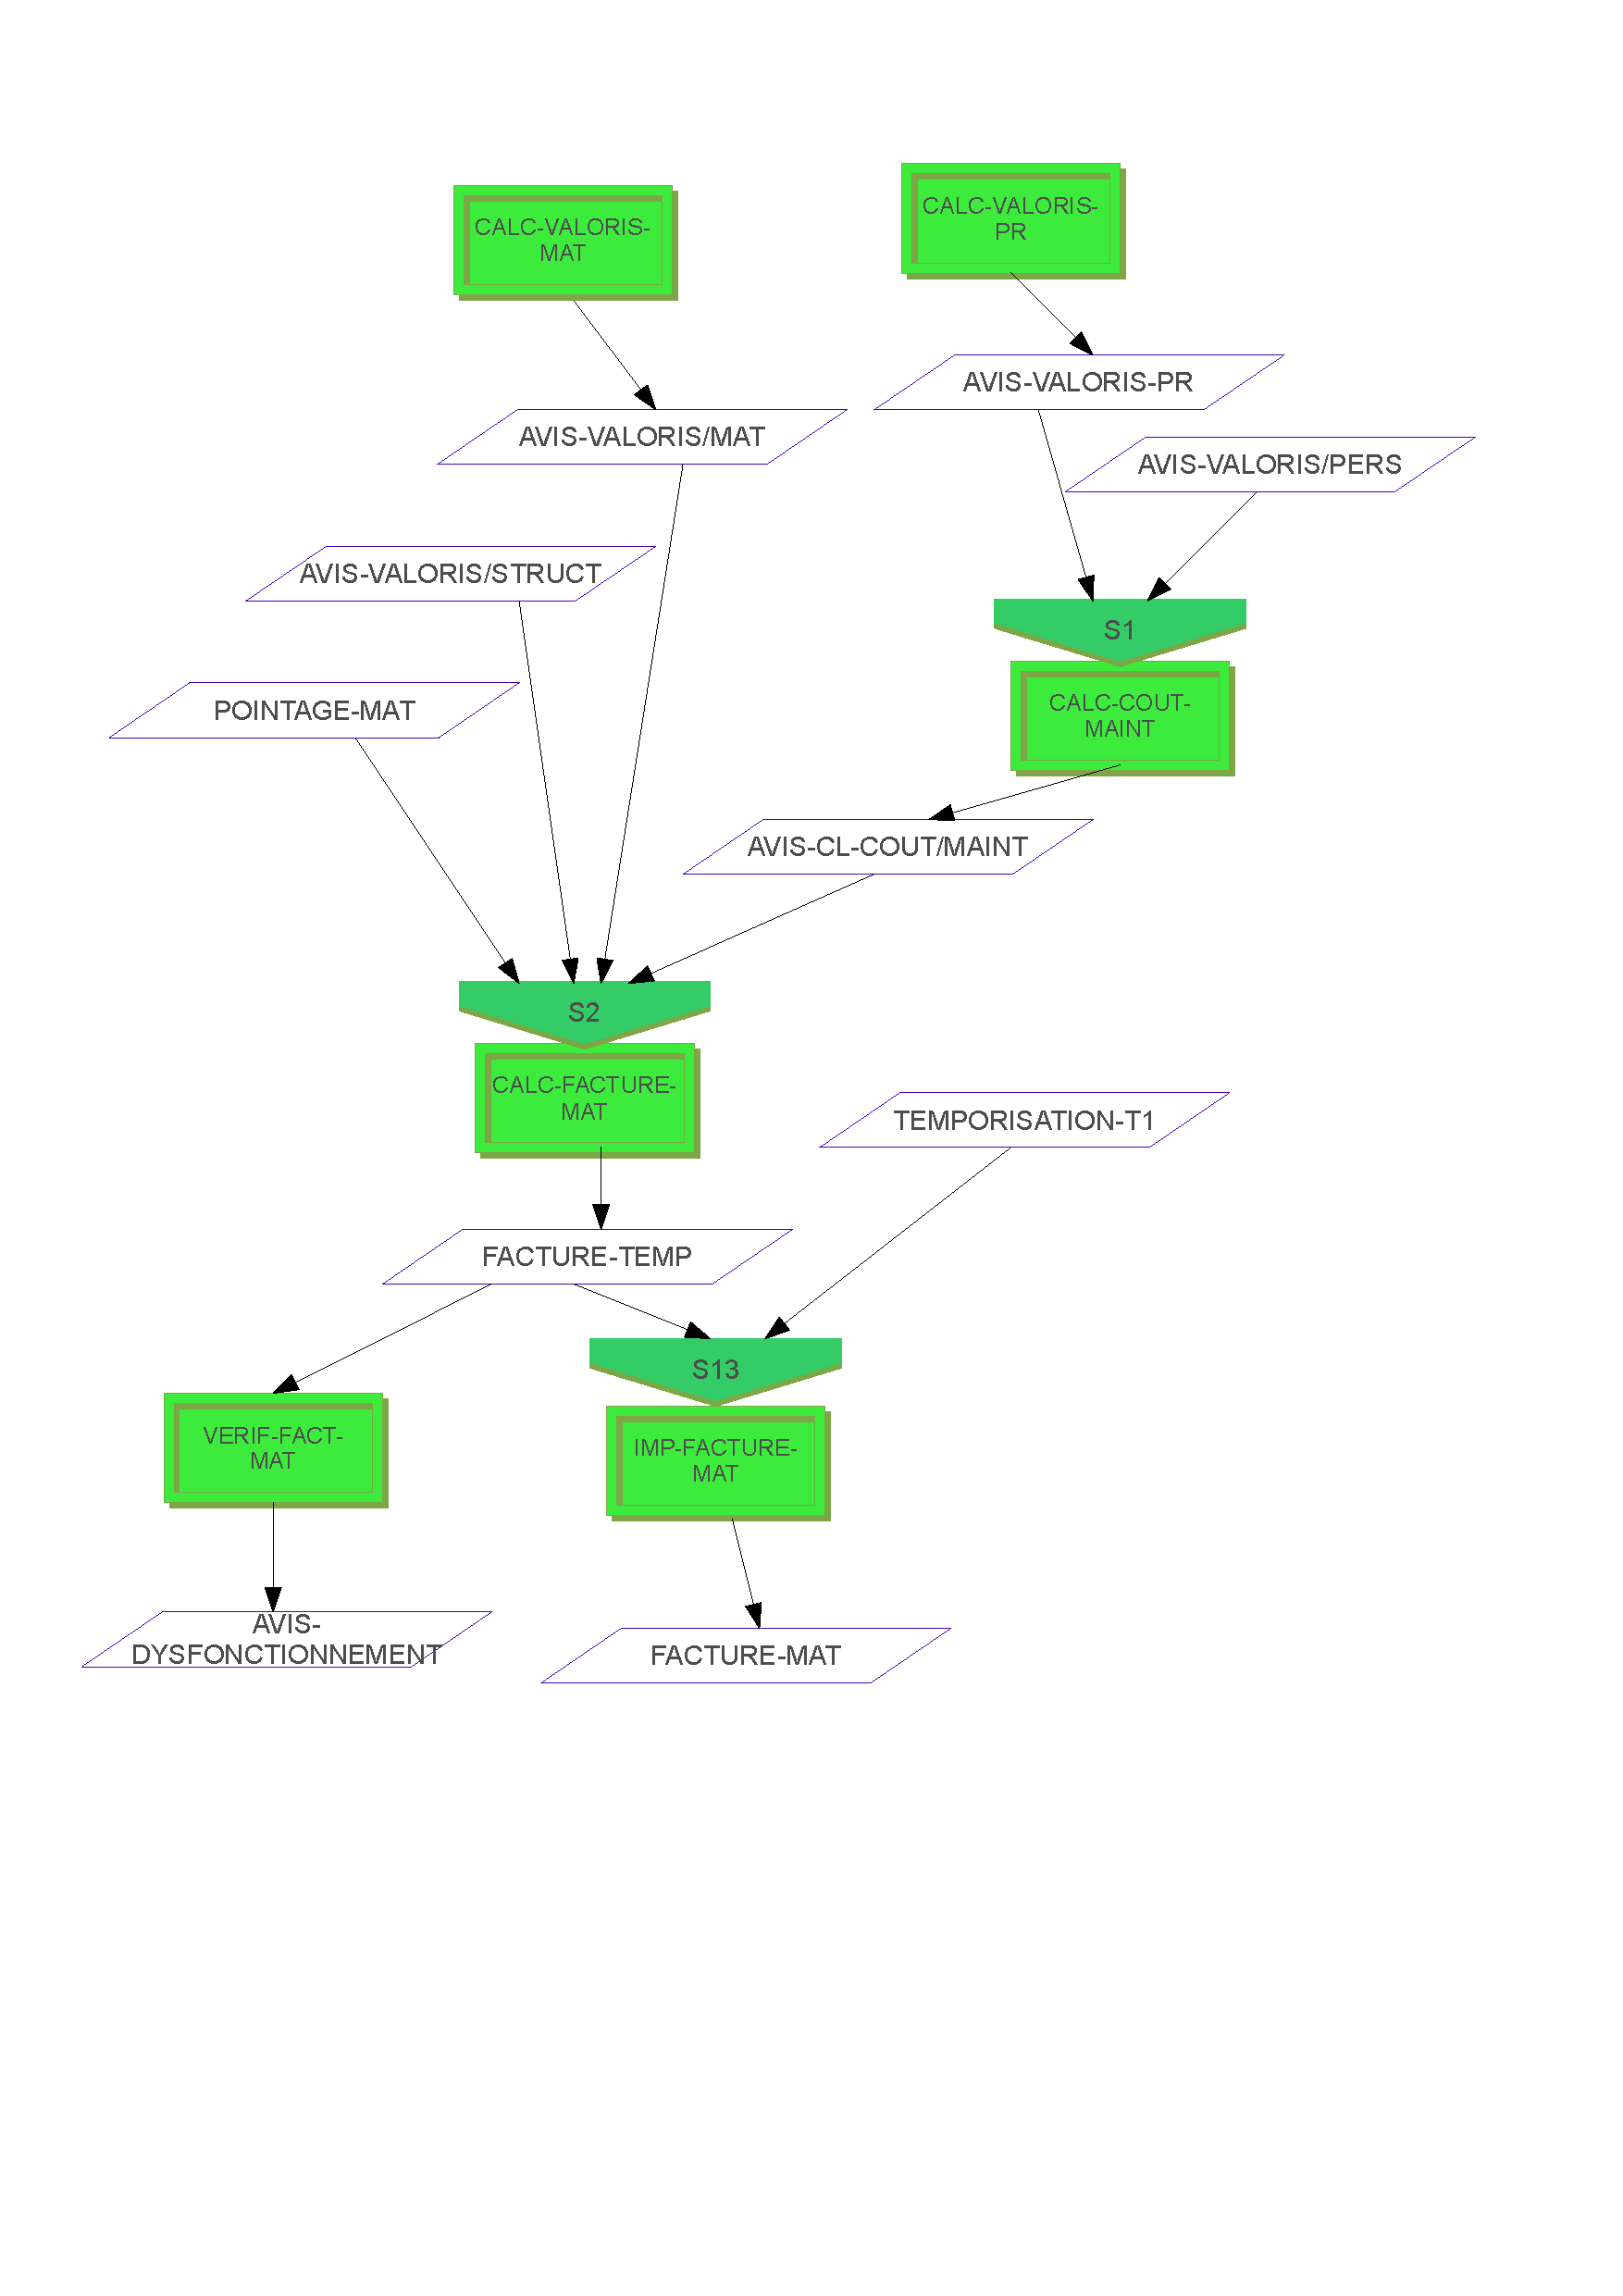
\includegraphics[width=0.9\textwidth]{Facturation.pdf}


                    %Ci-dessous le modèle organisationnel de traitement (MOT). --> 
                    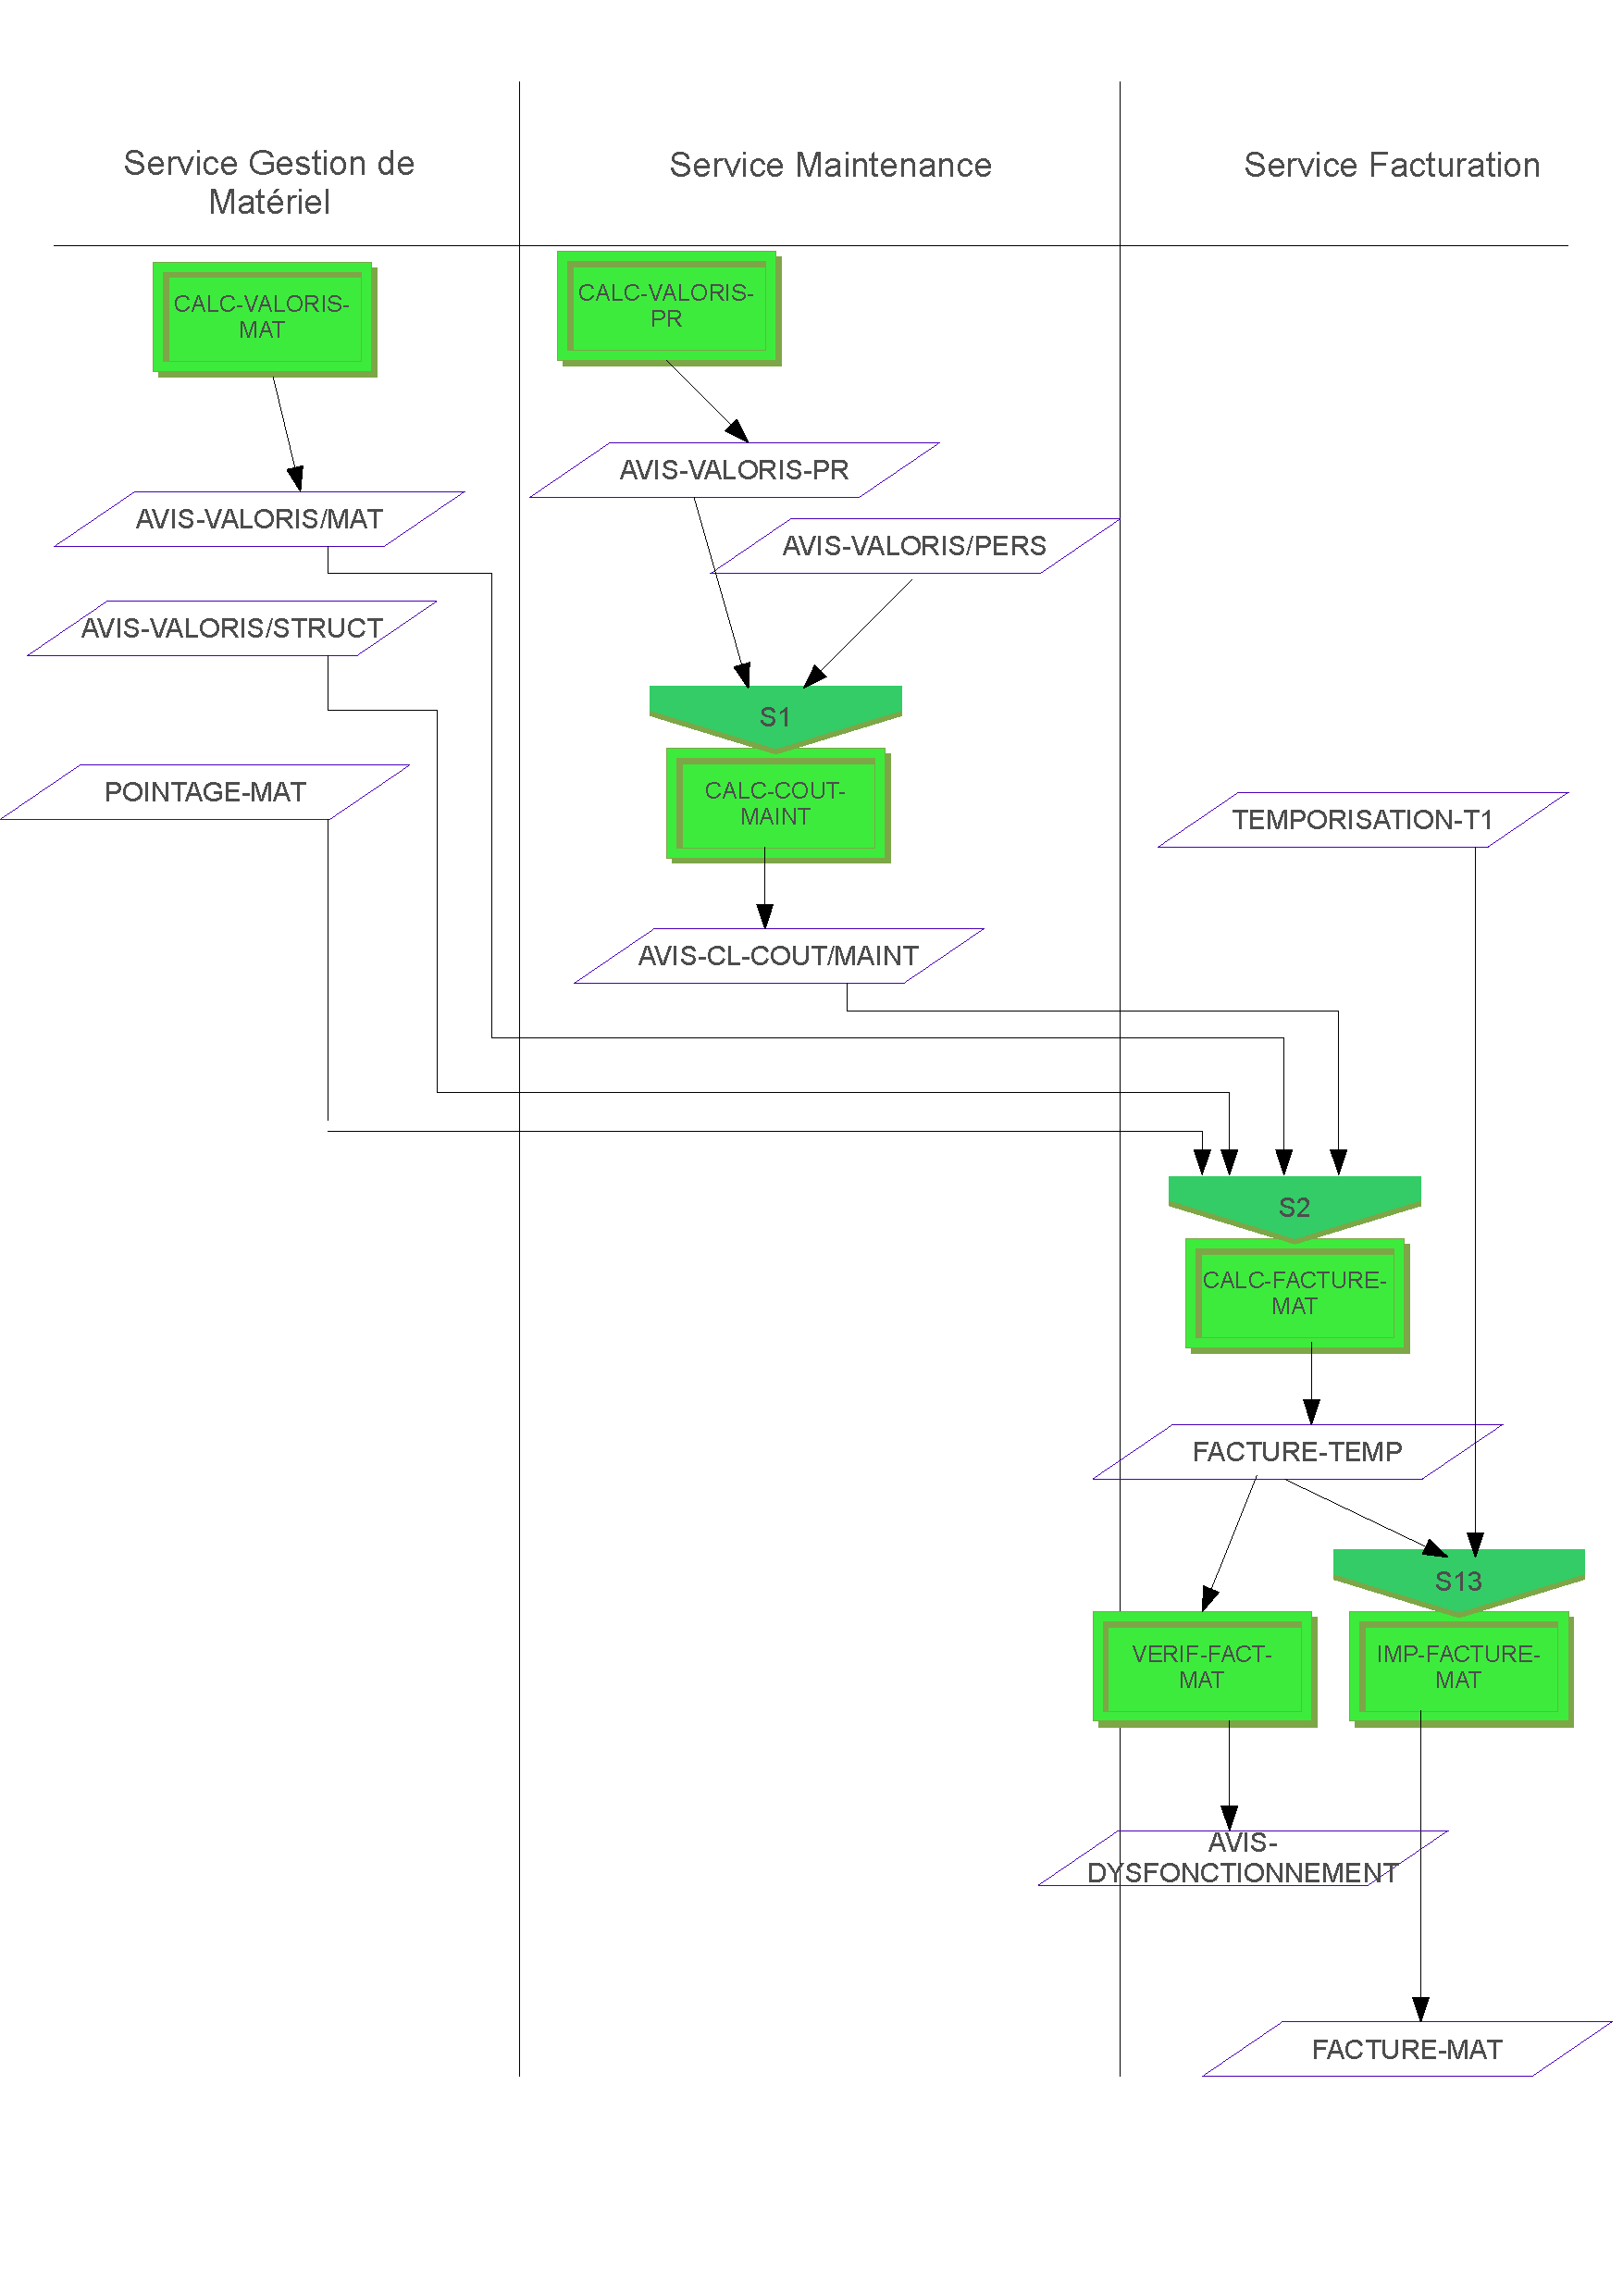
\includegraphics[width=0.9\textwidth]{MOTFacturation.pdf}


                \subsubsection{Processus Maintenance}
                    %Ci-dessous le modèle conceptuel de traitement (MCT) --> 
                    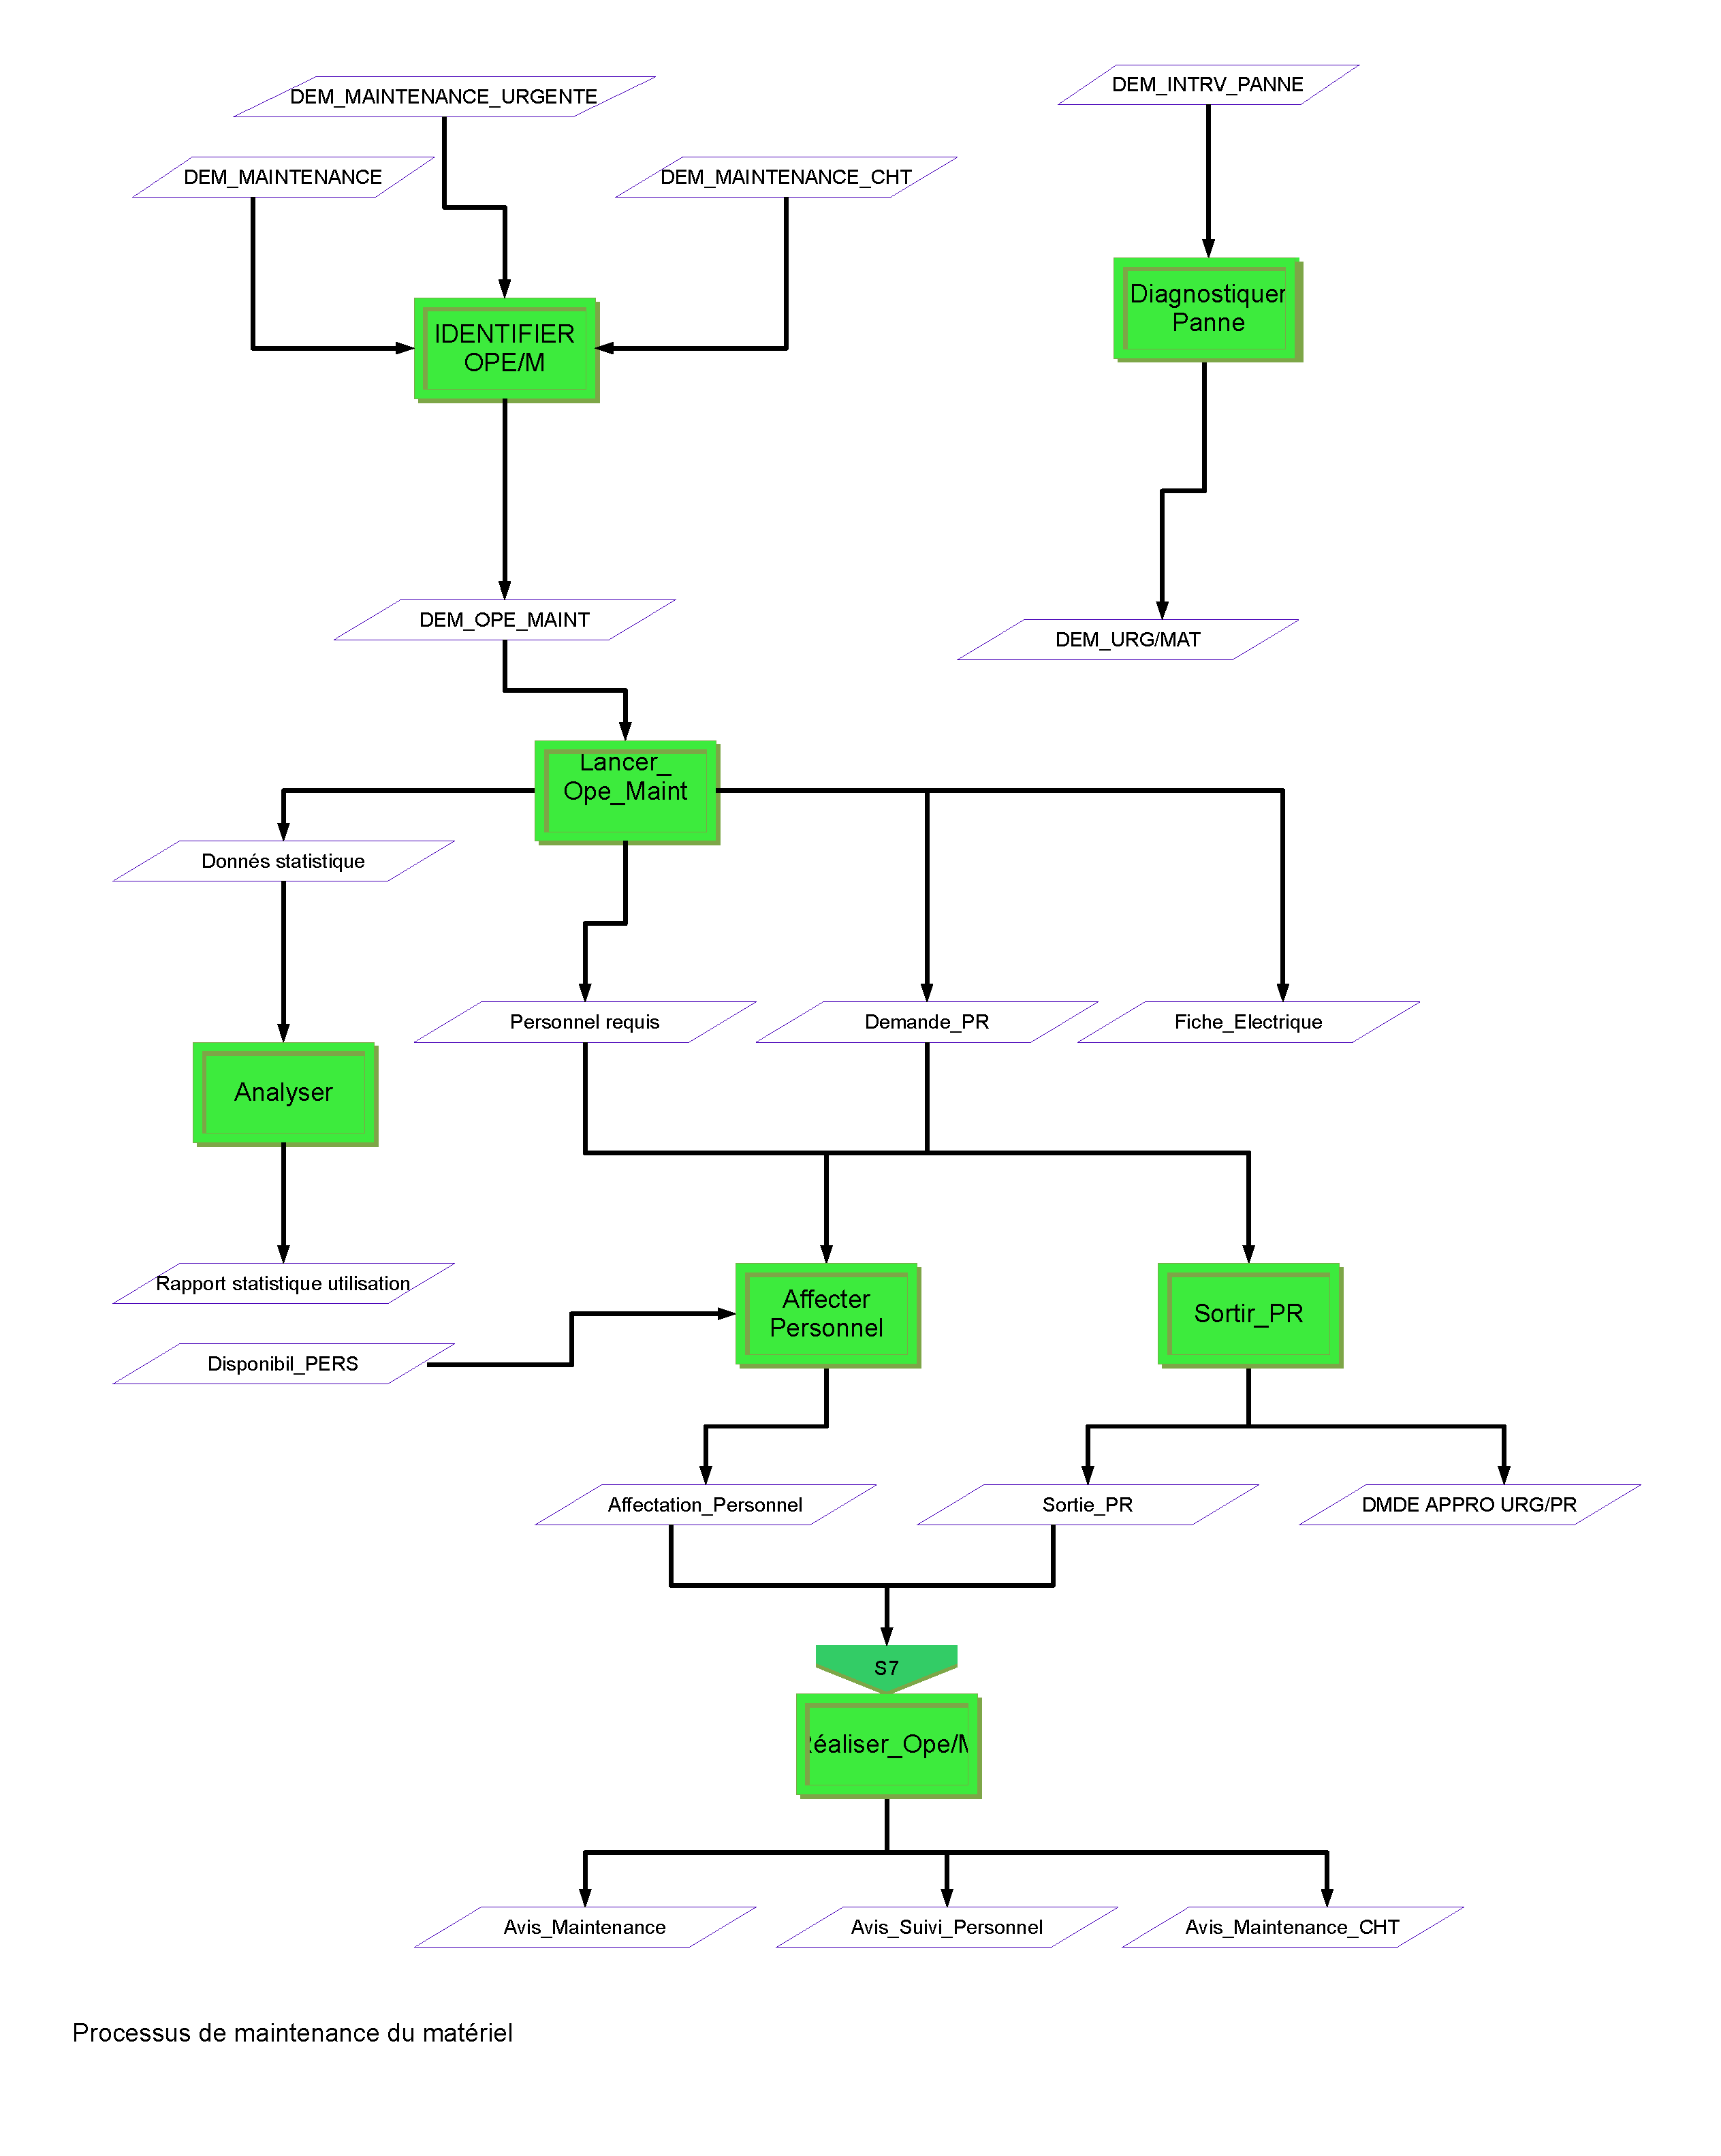
\includegraphics[width=0.9\textwidth]{MCT.pdf}


                    %Ci-dessous le modèle organisationnel de traitement (MOT)  --> 
                    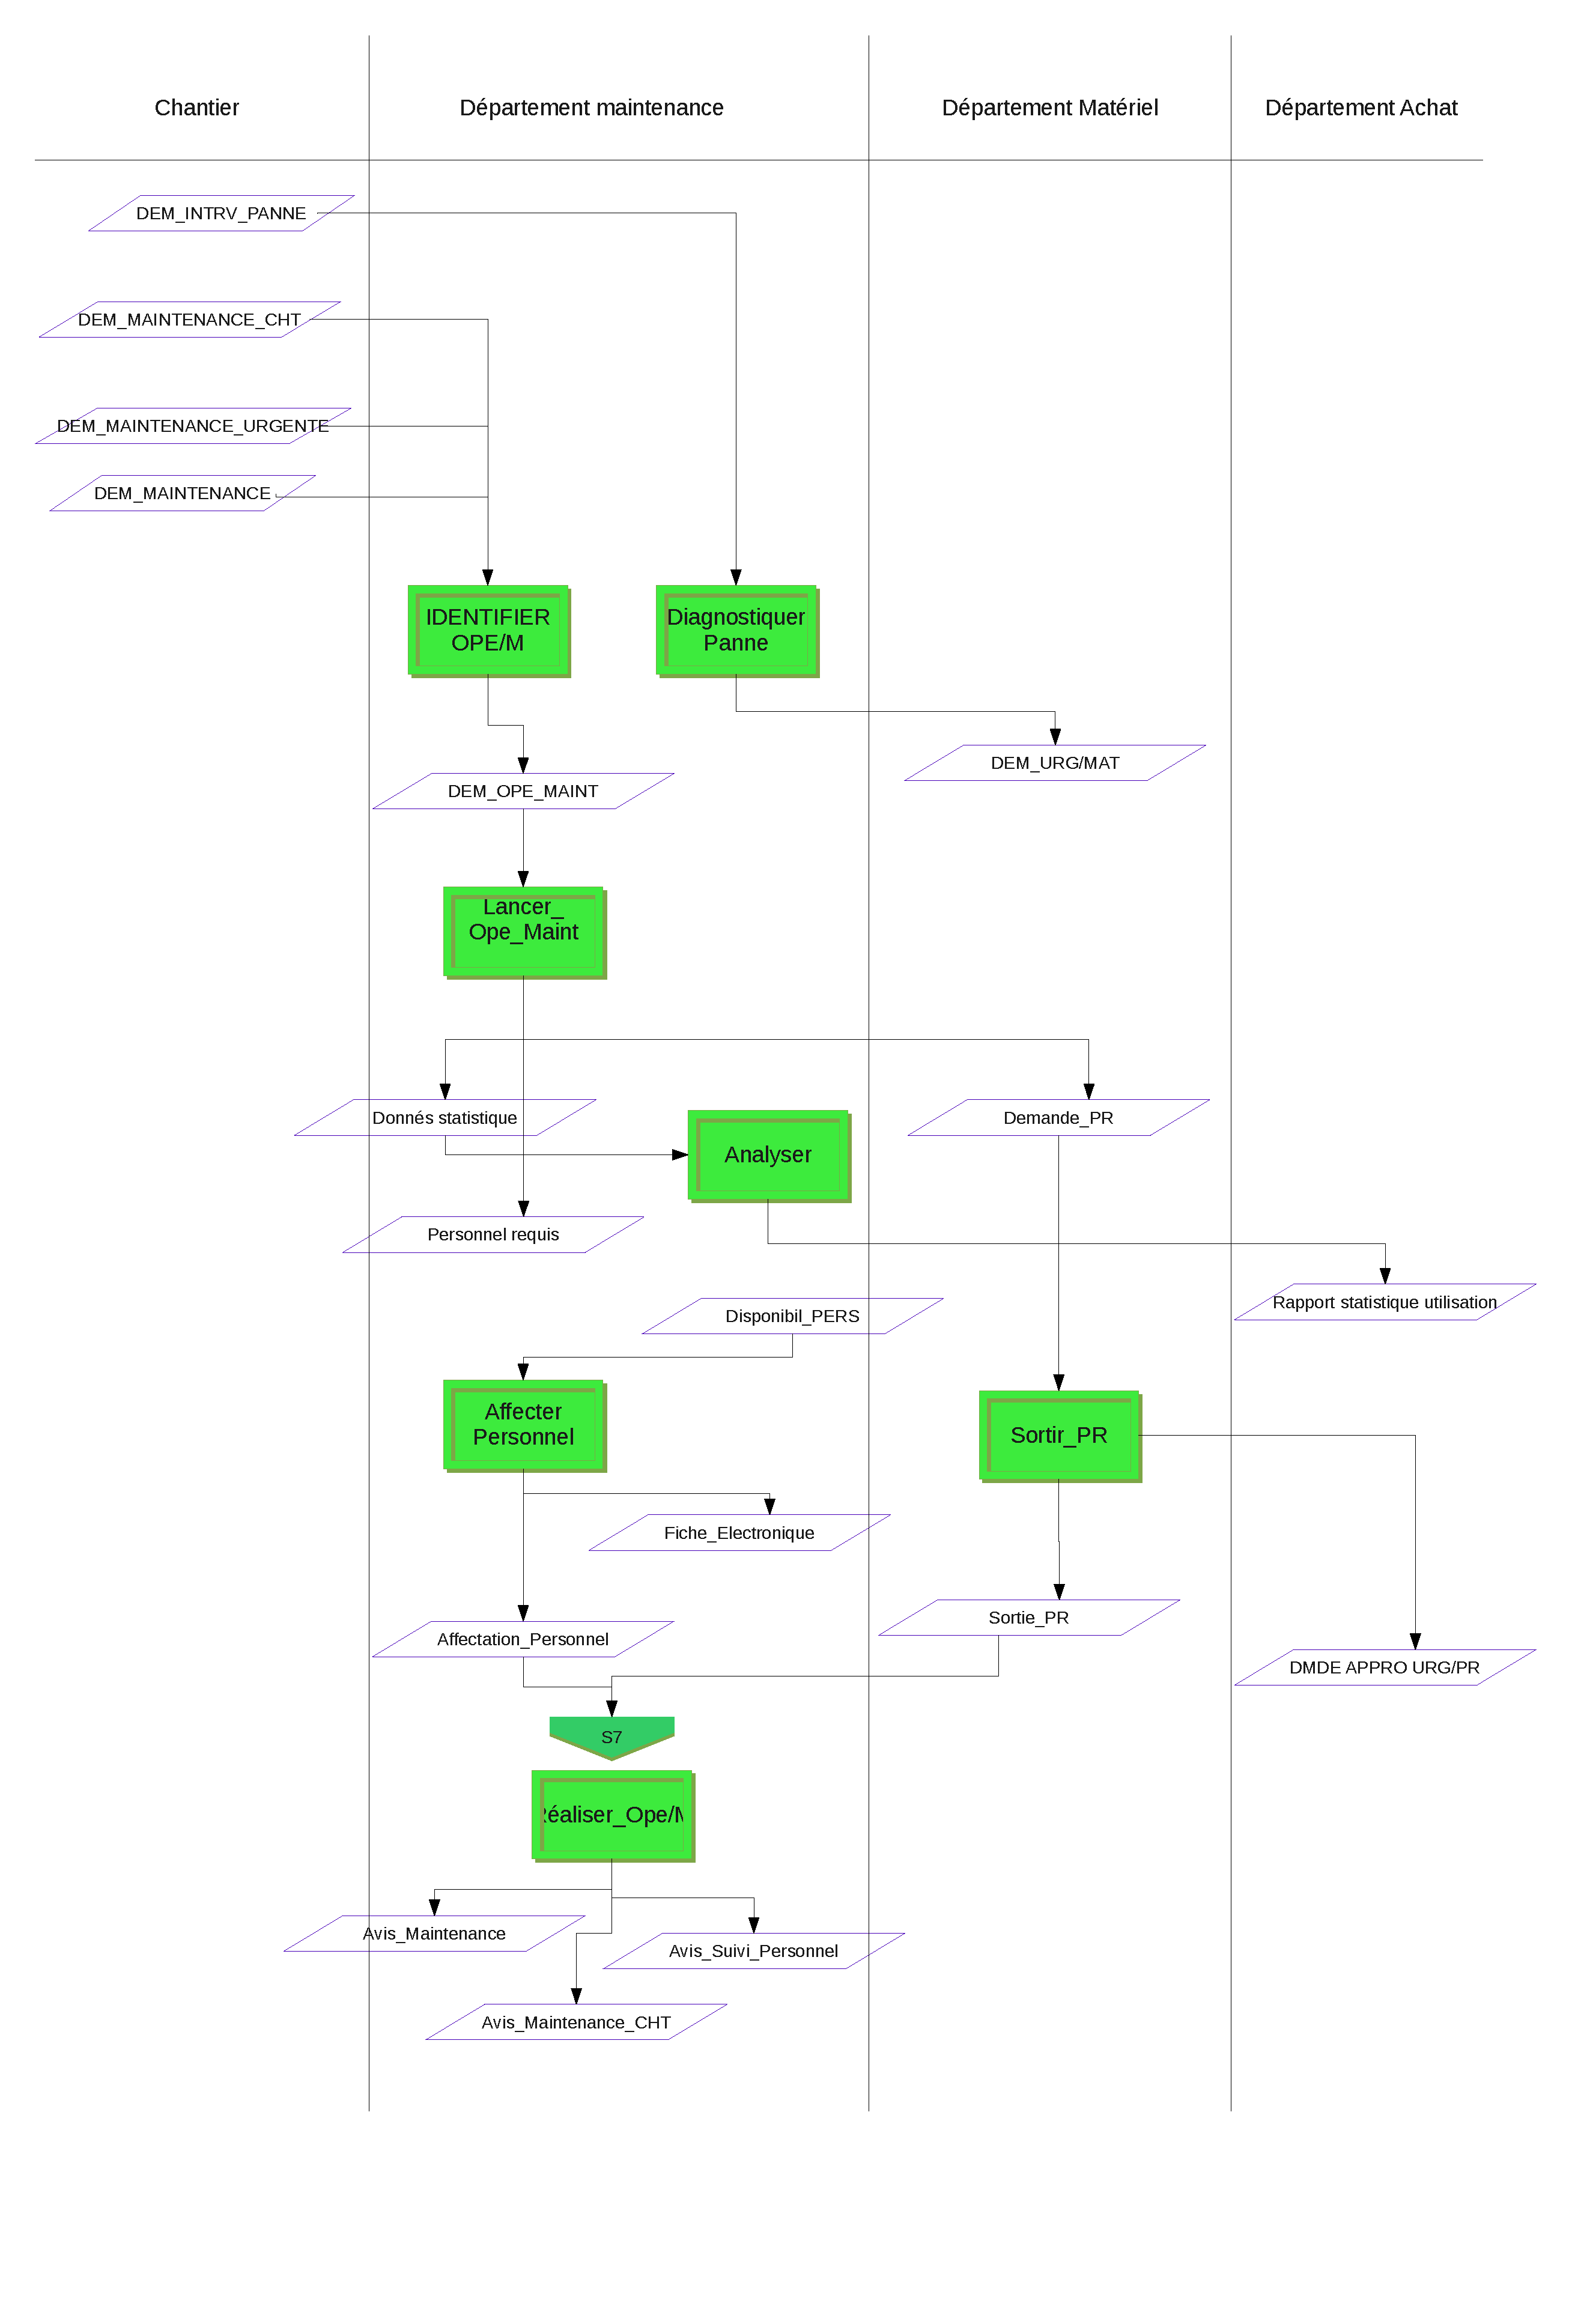
\includegraphics[width=0.9\textwidth]{MOT.pdf}

